\section{Grundlagen}\raggedbottom
\label{sec:Grundlagen}
In diesem Kapitel beschäftigen wir uns mit den theoretischen Grundlagen der Methoden, die benutzt wurden, um die Kundendaten zu analysieren. Dafür wollen wir zunächst die Syntax der Logfiles beschreiben. Das dient als Vorbereitung für den Abschnitt über die Mustererkennung. In diesem werden die verschiedenen Phasen der Mustererkennung beschrieben sowie die Methoden, die im weiteren Verlauf der Arbeit angewendet werden.

\subsection{Syntax der Logeinträge}
\label{sub:Aufbau der Logeinträge}
Das IFP generiert bei seiner Benutzung mehrere verschiedene Logfiles. Je nach Art des Logfiles können hier verschiedene Informationen gespeichert werden wie z.B. Zeitstempel, UserIDs, Exception Messages usw. Da für diese Arbeit aber nur die sog. \textit{Sessionlogs} relevant sind, soll auch nur deren Syntax beschrieben werden.\\
Die Einträge in den Sessionlogs spiegeln im Großen und Ganzen die Serveraktivität wider: Es werden ein- und ausgehende HTTP Requests festgehalten. Allerdings ist es nicht ausreichend nur eine Liste von Requests zu speichern. Sie müssen noch in einen gewissen Kontext gebracht werden. Deshalb werden zusätzlich zu den Requests auch Daten wie Zeitstempel, UserID, Parameter u.s.w. geloggt. Durch diese Informationen kann man nun nachvollziehen, welcher User zu welchem Zeitpunkt Daten gesendet bzw. angefragt hat. Neben der UserID wird auch die Session~ID mit geloggt. Sobald sich ein User erfolgreich in das IFP einloggt, wird eine SessionID generiert. Diese Session\-ID ist vom Zeitpunkt des Logins bis zum Logout gültig. Möchte sich derselbe User nach dem Logout direkt noch einmal einloggen, wird eine neue Session~ID generiert.\\
Die Einträge in den Logfiles können grob in die folgenden Felder unterteilen werden:\\

\begin{center}
	\begin{tabular}{c}
		\begin{lstlisting}[numbers=none, basicstyle=\scriptsize,caption=Felder in Sessionlogs,captionpos=b,label=lst:tab_session_fields]
[Timestamp] [Loglevel] [SessionID] [CustomerID] [UserID] [TaskID] [HTTP Request]
		\end{lstlisting}
		%\label{lst:tab_session_fields}
	\end{tabular}
\end{center}

Da nun die Syntax der Einträge erkannt wurde, kann die Mustererkennung beginnen.


\subsection{Mustererkennung}
\label{sub:Mustererkennung}
Nach \citet{BeKe19} lässt sich die Mustererkennung auch \textit{Data Mining} nennen. Data Mining ist wiederrum Teil eines Prozesses, der sich \textit{Knowledge Discovery in Databases} (KDD) nennt. Diesen Prozess haben \citet{BeKe19} in acht Schritte aufgeteilt.\\
Allgemeiner lässt sich aber die Mustererkennung auch auf andere Bereiche anwenden. Beispiele dafür wäre die Mustererkennung in Bilddateien \citep{DuHaSt01}. Da wir durch die Einleitung in Kapitel \ref{sec:Einleutung} bereits eine Schritte des KDD-Prozesses abgedeckt haben, werden im weiteren Verlauf der Arbeit die Phasen nach \citet{Wa11} beschrieben. Der Vollständigkeit halber werden die Phasen nach \citet{BeKe19} in Klammern aufgeführt. Da die Aufteilung nach \citet{Wa11} allerdings kompakter ist, wird diese im weiteren Verlauf angewendet.
\begin{enumerate}
	\item Segmentiereung (Datenauswahl / Datenbereinigung)
	\item Feature Extraction (Datenreduktion und -projektion)
	\item Klassifizierung (Modellfunktionalität / Verfahrensauswahl / Data Mining)
\end{enumerate}
\begin{comment}	
	Generell kann man in vielen verschiedenen Medien Muster erkennen, wie z.B. Bilddateien, Musikdateien oder eben in Textdateien. Dabei kommt es im Wesentlichen darauf an, welche Muster man erkennen möchte. So könnte man einem Programm beibringen, bestimmte Fischarten auf Fotos zu erkennen \citep{DuHaSt01}. Ein allgemeiner Ansatz, das Problem der Mustererkennung zu lösen, ist es, das Problem in folgende Teilprobleme aufzuteilen \citep{Wa11}:
Nach \citet{BeKe19} kann man die Mustererkennung auch als Data Mining beschreiben. In ihren Ausführungen beschreiben sie andere, aber ähnliche Phasen wie \citet{Wa11}. So lassen sich die drei Phasen auch mit den folgenden Begriffen benennen:
\begin{itemize}
	\item 
\end{itemize}
%An dieser Stelle wollen wir darauf hinweisen, dass diese Begriffe eher konzeptionell zu verstehen sind, anstatt wörtlich. Im Folgenden wird dieses generelle Vorgehen auf die Einträge der Logfiles angewendet. 
\end{comment}

\subsubsection{Segmentierung}
\label{ssub:Segmentierung}

In dem Schritt der Segmentierung wird festgestellt, welche Informationen aus den Logfiles für die Fragestellung relevant sind \citep{DuHaSt01}. Greifen wir dafür zunächst einmal die Definition aus der Einleitung auf, was es bedeutet ein Widget zu benutzen. Wie bereits erwähnt reicht ein pures Anzeigen von Informationen nicht aus; das Widget muss auch angeklickt werden. Ein Klick auf ein Widget hat i.d.R. immer denselben Effekt: man wird auf eine (evtl. vorgefilterte) Seite weitergeleitet. Das heißt, man sendet einen HTTP Request an den Server und der Server sendet eine Antwort. Also ist es offensichtlich, dass wir für unsere Analyse nur die HTTP Requests betrachten müssen und die Antworten des Servers irrelevant sind. Demnach sind nur Einträge von Interesse, die in dem Feld [HTTP Request] aus Listing \ref{lst:tab_session_fields} mit \textit{Incoming Request} anfangen. Dadurch wird die Menge an Einträgen, die wir betrachten wollen, um ca. die Hälfte reduziert.\\
Betrachten wir nun den Rest des Feldes genauer anhand eines Beispieleintrags, in dem ein Widget benutzt wurde. Insbesondere die URL ist für uns von Interesse:\\
%\\
\begin{lstlisting}[style=base,numbers=none,caption = Beispiel URL,captionpos=b,label=lst:url-beispiel]
/MULTIVERSA-IFP/lightning/ecm/liquidity/banks/liquidity\_banks.jsf?selectedView=ecm.liquidity.banks.view.all\&viewType=0\&@widget=LiquidityByBanksWidgetContent@\&banks=RpBLVhy85c5u4nGKeISH0A\&conversationContext=3\&\_ns\_=f63a91bc-9ab1-472d-bcb0-b6771837ffaa3\&\_nc\_=
\end{lstlisting}
%\label{lst:url-beispiel}
%\\
%\\
Der Name des Widgets ist in der URL erkennbar, wie man hier rot markiert sehen kann.\\
Neben dem HTTP Request sind diese weiteren Felder von Relevanz:\\
\begin{itemize}
	\item Timestamp
	\item SessionID
	\item UserID
\end{itemize}

\subsubsection{Feature Extraction}
	\label{ssub:Feature_extraction}
Nachdem alle irrelevanten Daten in der Segmentierung eliminiert wurden, ist der nächste Schritt die Feature Extraction. Dieser Begriff könnte irreführend wirken, da in dieser Arbeit keine Features im wörtlichen Sinne extrahiert werden, vielmehr werden die Daten in eine bestimmte Struktur transformiert \citep{BeKe19}. Diese besteht aus drei Mengen, die Menge an Usern, die Menge an SessionIDs und die Menge an Widgets. Von nun an wird diese Struktur \textit{Session Entity} genannt. Zu einem User gehört eine Menge an SessionIDs. Diese ist verknüpft mit den Widgets, die in dieser Session benutzt wurden. Mit anderen Worten beinhaltet eine Session Entity die Informationen, welche Widgets in einer Session von wem benutzt wurden. Abbildung \ref{fig:session-entity} soll diesen Zusammenhang verdeutlichen.\\
\begin{figure}[htb]
\begin{center}
	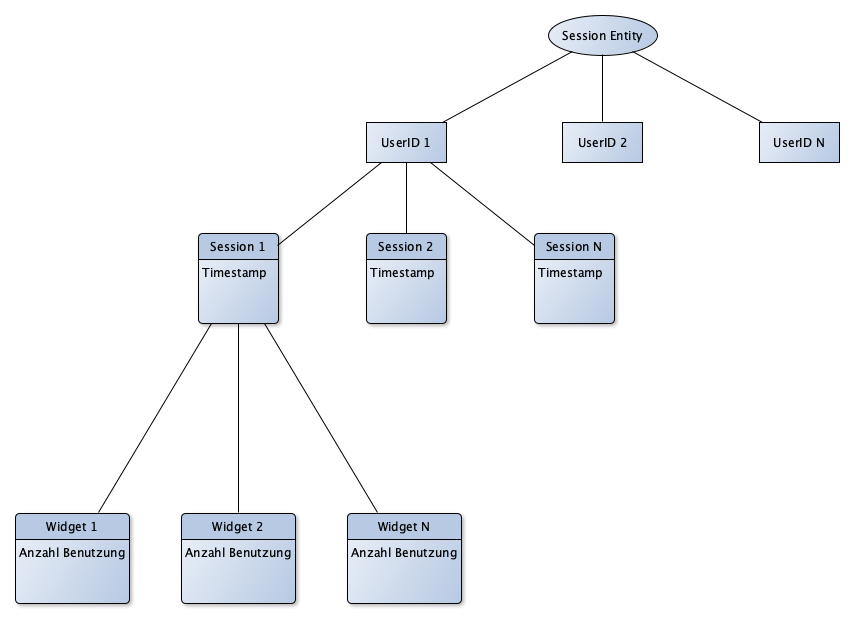
\includegraphics[width=\textwidth]{bilder/session-entity.png}
\end{center}
\caption{Session Entity}
\label{fig:session-entity}
\end{figure}

Zusätzlich zu der Information, welche Widgets benutzt wurden, wird noch festgehalten, wann eine Session beginnt und endet. Sowohl die Uhrzeit als auch die UserID werden im weiteren Verlauf der Arbeit keine tragende Rolle mehr spielen. Allerdings macht es Sinn diese Daten mitzuspeichern, da sie für zukünftige Anwendungsfälle relevant sein könnten.
%Prinzipiell gäbe es noch die Menge an time stamps, nach diesen wird aber nicht sortiert.

\subsubsection{Klassifizierung}
\label{ssub:Klassifizierung}
Nachdem die Daten transformiert sind, werden sie im nächsten Schritt analysiert. In Abschnitt \ref{sub:Problemstellung} wurde bereits erwähnt, dass in dieser Arbeit die Frage nach dem Zeitraum der Nutzung der Widgets und dem Workflow zu erörtern sind. Deshalb wird das weitere Vorgehen für beide Fragen gesondert dargestellt.
%Nun da die Daten transformiert wurden können wir beginnen die Daten zu klassifizieren. 
%Da wir in Abschnitt \ref{sub:Problemstellung} verschiedene Fragen beantworten wollen, müssen wir dafür die Klassifizierung für diese beiden gesondert betrachten.
%\\
\subsubsubsection{Diagramm}\\
%\\
Um die Frage zu klären, wie sich die Widgetnutzung pro Tag verhält, wird ein Linienhistogramm erstellt. Das hat den Vorteil, dass nicht nur die Nutzung an sich dargestellt wird, sondern auch ein Verlauf bzw. ein Trend in der Nutzung der Widgets. Zusätzlich wird in einem Tortendiagramm die anteilige Widgetnutzung dargestellt.
%\\
\subsubsubsection{Assoziationsregeln}\\
In dem folgenden Abschnitt werden die theoretischen Grundlagen zur Bestimmung von Assoziationsregeln vorgestellt. Zunächst sei aber drauf hingewiesen, dass dieser Abschnitt zu großen Teilen auf den Ausführungen von \citet{EsSa00} in \glqq\textit{Knowledge Discovery in Databases}\grqq{} basiert. Andere Quellen, die zur Erstellung des Abschnitts benutzt wurden, sind entsprechend gekennzeichnet.\\
%\\
Die Suche nach Assoziationsregeln wird auch oft als Warenkorbanalyse bezeichnet. Dabei geht es darum, in einer Datenbank Beziehungen zwischen den Daten zu finden. Bevor wir in die Theorie hinter den Assoziationsregeln eintauchen, wollen wir mit Hilfe der folgenden Tabelle die wichtigsten Begriffe vorstellen. Zum besseren Verständnis zeigen wir zu den Begriffen, die eingeführt werden, Analogien zu unserem Anwendungsfall und eines Online Shops.
\clearpage
\begin{table}[htb]
	\begin{center}
		\begin{tabular}{p{4cm}|l|p{5cm}}
			Allgemein & Online Shop & IFP\\
			%\hline
			%Datenbank & Die Menge aller Warenkörbe & Die Menge aller SessionIDs\\
			\hline
			Transaktion & Ein einzelner Warenkorb & Eine einzelne SessionID\\
			\hline
			Menge aller Transaktionen $D$ & Menge aller Warenkörbe $D$ & Menge aller SessionIDs $D$\\
			\hline
			Item & ein Produkt & ein Widget bzw. eine Widgetnutzung\\
			\hline
			Menge aller Items $I$ & Menge aller Produkte $I$ & Menge aller Widgets $I$
		\end{tabular}
		\caption{Begriffe zu Assoziationsregeln}
		\label{tab:begriffe_ar}
	\end{center}
\end{table}

Nun wollen wir definieren was eine Assoziationsregel ist. Betrachten wir dafür die Widgets $w_1$ und $w_2$. Eine Assoziationsregel wird mit \begin{equation*}w_1 \rightarrow w_2\end{equation*} notiert und sagt aus, dass wenn $w_1$ benutzt (also angeklickt) wird, $w_2$ auch benutzt wird. An eine Assoziationsregel sind zwei Werte geknüpft, die beschreiben, wie \glqq gut\grqq{} eine Regel ist: der \textit{Support} und die \textit{Konfidenz}. Diese Werte wollen wir mit Hilfe eines kurzen Beispiels definieren:\\

		\begin{table}[htb]
	\begin{center}
		\begin{tabular}{|l|l|}
			\hline
			SessionID&Benutzte Widgets\\ \hline
			1& $w_1,w_2,w_4,w_5$\\ \hline
			2& $w_1,w_3$\\ \hline
			3& $w_2,w_5$\\ \hline
			4& $w_1,w_2$\\ \hline
			5& $w_2,w_3,w_5$\\ \hline
		\end{tabular}
		\caption{Beispiel Datenbank zu Assoziationsregeln}
		\label{tab:bsp_ar}
	\end{center}
\end{table}

%\newpage
%Wir wollen zunächst die Begriffe aus Tabelle \ref{tab:begriffe_ar} auf dieses Beispiel anwenden:
Zunächst werden die Begriffe aus Tabelle \ref{tab:begriffe_ar} auf das Beispiel der Datenbank (vgl. Tabelle \ref{tab:bsp_ar}) angewendet:
\begin{itemize}
	\item Die Menge aller Items $I = \{w_1, w_2, w_3, w_4, w_5\}$. Eine Menge $X \subseteq I$ wird auch \textit{Itemset} genannt. Also wäre z.B. $\{w_1, w_3\} \subseteq I$ ein Itemset.
	\item Die Menge aller SessionIDs $D = \{1,2,3,4,5\}$. $T_i$ mit $i \in D$ und $T_i \subseteq I$. Demnach gilt z.B. $T_1 = \{w_1,w_2,w_4,w_5\}$
\end{itemize}

Der Support einer Menge wird definiert als:\\

\begin{equation*}
	\text{support(X)} = \frac{\text{Anzahl der Transaktionen, die X enthalten}}{\text{Anzahl aller Transaktionen}}, \text{ X} \subseteq I
\end{equation*}\\

Demnach gilt z.B. für X$_1$ =  $\{w_1,w_3\}$, X$_2$ = $\{w_2\}$ und X$_3$ = $\{w_1\}$:\\
\begin{equation*}
	\begin{split}
		\text{support(X$_1$)} = \frac{1}{5} = 0.2 ,\text{ support(X$_2$)} = \frac{4}{5} = 0.8, \text{ support(X$_3$)} = \frac{3}{5} = 0.6
		%\text{support(X$_1$)} = \frac{1}{5} = 0.2\\
		%\\
		%\text{support(X$_2$)} = \frac{4}{5} = 0.8\\
		%\\
		%\text{support(X$_3$)} = \frac{3}{5} = 0.6\\
	\end{split}
\end{equation*}

Der Support eines Itemsets beschreibt demnach die relative Häufigkeit des Itemsets, im Bezug auf die Anzahl der Transaktionen in der Datenbank \citep{BeKe19}. Desweiteren gilt für X,Y $\subseteq$ I:\\
\begin{equation*}
	\text{support(X $\rightarrow$ Y)} = \text{support(X $\cup$ Y)}
\end{equation*}

Als nächstes wollen wir die Konfidenz definieren. Die Konfidenz einer Assoziationsregel X $\rightarrow$ Y ist definiert als:\\
\begin{equation*}
	\text{konfidenz(X $\rightarrow$ Y)} = \frac{\text{support(X $\rightarrow$ Y)}}{\text{support(X)}}
\end{equation*}

Auf Tabelle \ref{tab:bsp_ar} bezogen wollen wir nun die Konfidenz für die Regel $\{w_1\} \rightarrow \{w_3\}$ berechnen. Es gilt:\\
\begin{align*}
	\text{konfidenz($\{w_1\} \rightarrow \{w_3\}$)} &= \frac{\text{support($\{w_1\} \rightarrow \{w_3\}$)}}{\text{support($\{w_1\}$)}}\\ \\
	&= \frac{\text{support($\{w_1\} \cup \{w_3\}$)}}{\text{support($\{w_1\}$)}}\\ \\
	&= \frac{0.2}{0.6} = 0.33
\end{align*}
Die Konfidenz beschreibt also wie hoch die Wahrscheinlichkeit ist, dass wenn $w_1$ benutzt $w_3$ auch benutzt wurde. \citep{BeKe19}\\

Nachdem wir alle relevanten Begriffe bzgl. der Assoziationsregeln definiert haben, wollen wir genauer erörtern, wie Regeln gefunden werden sollen. Dazu rufen wir uns noch einmal ins Gedächnis, welche Information wir uns aus den Regeln erhoffen: wir wollen Workflows erkennen. Nehmen wir mal an, das Itemset $\{w_1,w_3\}$ käme in einer Datenbank mit 1000 Einträgen nur ein einziges Mal vor, ist es offentsichtlich, dass man bei dieser Regel nicht von einem Workflow sprechen kann. Das bedeutet wir suchen Itemsets, die \textit{häufig} vorkommen. Diese Häufigkeit wird durch den \textit{minsupport} festgelegt. Ein Itemset gilt als häufig, wenn gilt:\\
\begin{equation*}
	\text{support(X)} \geq \text{minsupport}
\end{equation*}

Analog wollen wir auch nicht alle Regeln, die wir aus den häufigen Itemsets generieren, betrachten. Vielmehr wollen wir die Regeln finden, die die \textit{minkonfidenz} erfüllen. Daraus folgt, dass man die Aufgabe in zwei Teilprobleme aufteilen kann:
\begin{enumerate}
	\item Finde alle Itemsets die häufig sind, also den minsupport erfüllen. Ein naiver Ansatz wäre, die Potenzmenge $\mathcal{P}$($I$) zu berechnen und zu prüfen, welche der Teilmengen den minsupport erfüllen. Allerdings hätte dieses Vorgehen eine Laufzeit von $\mathcal{O}(2^n)$ wobei n die Anzahl der Widgets ist. Deshalb wird der sog. \textit{Apriori Algorithmus} verwendet, der die Laufzeit stark einschränkt, indem die zu betrachtenden Itemsets eingeschränkt werden.\\
	\item Finde alle Assoziationsregeln, die aus den häufigen Itemsets generiert werden können und die die minkonfidenz erfüllen. Wenn Itemset X häufig ist, ist auch jede Teilmenge A von X häufig und ergibt die Regel A $\rightarrow$ X $-$ A. Für diese Regeln muss die Konfidenz geprüft werden.
\end{enumerate}

Bevor wir nun die Algorithmen vorstellen, die zur Lösung der Teilprobleme benutzt wurden, sei noch angemerkt, dass der minsupport und die minkonfidenz Werte sind, die vom Benutzer festgelegt sind.
%\\
\subsubsubsection{Apriori Algorithmus}\\
%\\
Der Apriori Algorithmus wurde von \citet{AgImSw93} entwickelt und wird benutzt, um möglichst effizient häufige Itemsets zu finden. Dabei wird folgendes Lemma ausgenutzt:
\begin{lemma}
	Sei X ein Itemset. Wenn X kein häufiges Itemset ist, ist auch keine Obermenge von X häufig. \citep{AgImSw93}
	\label{lem:sets}
\end{lemma}
Ausgangspunkt der Kandidatengenerierung ist, dass man häufige Itemsets mit $k$ Elementen betrachtet. Aus diesen Itemsets sollen nun Itemsets generiert werden, die $k+1$ Elemente beinhalten. Um das zu erreichen, werden zwei Itemsets vereinigt, die $k-1$ gleiche Elemente haben. Angenommen, wir hätten die häufigen Itemsets $X = \{w_1, w_2, w_3\}$ und $Y = \{w_1, w_2, w_4\}$. Beide Mengen haben $k=3$ Elemente. Um aus diesen Mengen eine $k+1=4$ - elementige Menge zu generieren, müssen sie $k-1=2$ gleiche Elemente haben. Da das der Fall ist, erhalten wir als Ergebnis die Vereinigung beider Mengen mit $X \cup Y = \{w_1, w_2, w_3, w_4\}$. Dieser Schritt wird \textit{join} genannt.\\
Nach dem join muss noch geprüft werden, ob der generierte Kandidat auch Lemma \ref{lem:sets} erfüllt. Dies geschieht beim \textit{pruning} indem geprüft wird, ob jede $k-1$ - elementige Teilmenge des generierten Kandidaten häufig ist. Denn wenn eine Teilmenge des generierten Kandidaten nicht häufig ist, kann dieser auch nicht häufig sein und muss nicht weiter betrachtet werden. In Anhang Teil \ref{anhang:zusatz1} wird die Kandidatengenerierung mit dem Beispiel aus Tabelle \ref{tab:bsp_ar} vorgerechnet.
%\\
\subsubsubsection{Assoziationsregeln finden}\\
%\\
Aus den häufigen Itemsets, die der Apriori Algorithmus gefunden hat, wollen wir nun Assoziationsregeln finden. Ähnlich wie bei den häufigen Itemsets wollen wir nur Regeln finden, die die minkonfidenz erfüllen. Das erreichen wir, indem aus einem häufigen Itemset X zunächst Regeln gebildet werden, die der Form 
\begin{equation*}
Y \rightarrow X - Y, Y \subset X
\end{equation*}
entsprechen. Ähnlich wie bei der Kandidatengenerierung nutzen wir wieder eine Teilmengenbeziehung aus: Wenn die Regel $Y \rightarrow X - Y$ die minkonfidenz nicht erfüllt, erfüllt auch keine Teilmenge $Y' \subset Y$ mit der Regel $Y' \rightarrow X - Y'$ die minkonfidenz.

\clearpage
